 \documentclass[12pt]{article} 
 \usepackage{amssymb}
\usepackage{amsmath}
\usepackage{amsthm}
\usepackage{float}
\usepackage{geometry}
\usepackage[backend=bibtex,style=alphabetic]{biblatex}
\usepackage{graphicx}
\graphicspath{ {./images/} }
\usepackage{caption}
\usepackage[utf8]{inputenc}
\newtheorem*{remark}{Izrek o prepovedi kloniranja}
\newtheorem{postulat}{Postulat}

\usepackage[slovene]{babel}
\usepackage{booktabs}
\setcounter{tocdepth}{2} % Show sections

\addbibresource{references.bib}
\geometry{
 a4paper,
 total={160mm,240mm}  
  }
  
 \begin{document}
 $~$ 
 
 \vspace{2cm}
 
 \centerline{\bf \huge   Kvantni denar}
 
 \vspace{1cm}
 
  \centerline{\huge  Luka Skeledžija}
  
   \vspace{1cm}
  
  \centerline{\large Mentor: prof. dr. Rok Žitko}
  
  \vspace{1cm}
  
  \centerline{\large Seminar, 3. letnik}
  
  \vspace{1cm}
  
  \centerline{\large Oddelek za fiziko, FMF, UL, 2022/2023}
  
  \vspace{6cm}
  
  \begin{minipage}[c]{0.9\hsize}
  {\bf Povzetek}
  
  V kvantni mehaniki srečamo nekatere fizikalne pojave, ki jih iz klasične fizike nismo vajeni. Čeprav čudna, nam takšna nova fizika omogoča razvoj tehnologij, ki v okviru klasične fizike ne bi bile mogoče. Takšen primer je izrek o prepovedi kloniranja, ki predstavlja teoretično osnovo za veliko družino kvantnih kriptografskih protokolov. V okviru tega seminarja preletimo osnovne koncepte kvantne informacijske teorije, izpeljemo in dokažemo izrek o prepovedi kloniranja ter z njegovo pomočjo teoretično varno rešimo problem ponarejanja denarja. 
    \end{minipage}

 
 \newpage
 
 \tableofcontents

 \newpage
  
  
 \section{Uvod}
	Zakaj imajo kovanci in papirnati bankovci v našem žepu kakršno koli vrednost? Kratek odgovor bi bil, da jim je vrednost in uporabo odredila zaupanja vredna institucija (npr. centralna banka po naročilu države) \emph{in hkrati} obstaja le omejena količina tako izdanih bankovcev in kovancev. Zaradi drugega pogoja je fizičen denar opremljen z različnimi varnostnimi elementi, ki močno otežujejo njihovo ponarejanje in varujejo vrednost valute. Ponarejanje v praksi je sicer \emph{težko}, vendar nas vedno zanimajo še boljše (in morda teoretično brezhibne) rešitve, ki se ne zanašanjo na otip papirja, hologramski, vodni, UV, infrardeči ter miniaturni tisk \cite{bankSecurityFeatures2018}.  V uporabi so tudi še bolj zanimive metode npr. digitalni filtri v orodjih kot so Adobe Photoshop in nekaterih tiskalnikih, ki onemogočajo procesiranje slik bankovcev \cite{SoftwareDetectionCurrency}. 

\subsection{Aktualne rešitve}
	
\par Zanimivo je, da nas pri plačevanju s kartico težave ponarejanja denarja očitno ne pestijo, saj se vse dogaja znotraj bančnega sistema, kjer avtentičnost denarja pred vstopom vanj preverijo. Vendar pa morajo biti tudi bančne kartice na nek način zaščitene pred neavtoriziranim kopiranjem. Vsaka kartica namreč vsebuje polprevodniški mikročip in sistem simetrične kriptografije - torej uporabljajo isti ključ za šifriranje in dešifriranje \cite{CS101IntroductionComputing}. Na čipu je shranjena kopija šifrirnega ključa, ki ob vsaki transakciji zakodira unikatno sporočilo (npr. dovolj dolg naključni niz ali današnjo časovno oznako, angl. timestamp), ki ga nato pošlje na banko, kjer hranijo kopijo šifrirnega ključa. Banka sporočilo dešifrira in s tem potrdi avtentičnost transakcije. Bistvo te sheme je, da šifrirni ključ polprevodniškega čipa nikoli ne zapusti, ampak s t.i. reševanjem unikatnih izzivov (šifriranjem nizov) banki dokazuje, da šifrirni ključ pozna \cite{CS101IntroductionComputing}. Ker je ključ shranjen znotraj izjemno majhnega kosa polprevodnika, je branje le-tega izjemno zahtevno \cite{christopheDescramblingDataReading2006} in zato za povprečnega ponarejevalca pretežko.
\par
V teoriji bi lahko vsak bankovec opremili s takšnim polprevodniškim elementom in tako potrjevali avtentičnost. Vendar je to po eni strani potratno, po drugi pa nas kvantna mehanika lahko pripelje še bližje tudi teoretično varnemu sistemu. 

\subsection{Kvantni denar}

Leta 1983 je Stephen Wiesner objavil članek v katerem predlaga shemo t.i. "Kvantnega denarja" \cite{wiesnerConjugateCoding1983}. V splošnem je Wiesnerjeva shema kvantni kriptografski protokol (zaenkrat še brez praktične implementacije), ki opisuje kako ustvariti in verificirati bankovce odporne na ponarejanje \cite{QuantumMoney2022}. Poleg unikatne serijske številke bi vsak bankovec opremili še z nizom izoliranih dvonivojskih kvantnih sistemov. Tedaj po Izreku o prepovedi kloniranja ni mogoče ustvariti identične in neodvisne kopije poljubnega neznanega kvantnega stanja, saj to krši osnovna načela kvantne mehanike (konkretno linearnost) \cite{NocloningTheorem2022}. Za vsak sistem v nizu dvonivojskih kvantnih sistemov obstaja verjetnost $3/4$ \cite{molinaOptimalCounterfeitingAttacks2012}, da bo kopija  neznanega stanja popolna \cite{QuantumMoney2022}. Če je število kvantnih sistemov v nizu enako $N$, je tedaj verjetnost za nastanek popolne kopije niza $(3/4)^N$. Upoštevamo, da je na niz na bankovcu dolg in tako za velike $N$ kaj hitro ugotovimo, da je verjetnost za slučajen nastanek popolne kopije celotnega niza eksponentno majhna. 

\section{Kvantna informacijska teorija}
\par Ker se Wiesnerjeva shema naslanja na poglavja iz kvantne informacijske teorije (npr. Izrek o prepovedi kloniranja), moramo za globlje razumevanje na tej ravni v nadaljevanju razložiti še nekaj idej s področja kvantne mehanike.

\subsection{Lastnosti kvantnih sistemov}

V klasični fiziki lastnosti sistema obstajajo neodvisno od meritve in so del realnosti. Meritev te lastnosti le razkrije. V kvantni mehaniki pa vektor stanja določa le verjetnosti, da bomo pri meritvi dobili določen rezultat. Dva delca, ki sta na začetku opisana z enakim vektorjem stanja, lahko ob isti meritvi vrneta dva različna rezultata. Kvantno mehaniko lahko razumemo kot matematično ogrodje za razvoj fizikalnih teorij, ki smo ga izoblikovali na podlagi več deset let fizikalnih eksperimentov in ugibanja, kako se obnaša narava na skali atomov in podatomskih delcev. Osnovni postulati kvantne mehanike tako predstavljajo povezavo med fizičnim svetom in matematičnim formalizmom.

\begin{postulat}
Kvantno stanje je element Hilbertovega prostora.
\end{postulat}

\begin{postulat}
V kvantni mehaniki opazljivkam ustrezajo hermitski operatorji.
\end{postulat}

\begin{postulat}
(Bornovo pravilo) Pri meritvi opazljivke $A$ v stanju $| \psi \rangle$ bomo dobili rezultat $\lambda_j$ z verjetnostjo $p_j = | \langle j | \psi \rangle |^2$.
\end{postulat}

\begin{postulat}
(Kolaps valovne funkcije) Če pri meritvi opazljivke $A = \sum_i \, \lambda_i \, | i \rangle \, \langle i |$ izmerimo vrednost $\lambda_i$, potem je takoj po meritvi sistem v lastnem stanju $| i \rangle$.
\end{postulat}

\begin{postulat}
Časovno spreminjanje kvantnega stanja opišemo z unitarnim operatorjem.
\end{postulat}
S tem smo postavili osnove matematičnega formalizma, s katerim bomo delali v nadaljevanju. \cite{zitkoKvantneRacunalniskeTehnologije2017}



\subsection{Kubit}
\label{kubit} 

\emph{Bit} je fundamentalni koncept klasičnega računalništva, klasične informacijske teorije in hkrati tudi najmanjša enota informacije. V kvantni mehaniki definiramo analogni koncept, kjer obravnavamo t.i. \emph{kubite}. Če v klasični informacijski teoriji pripišemo bitu eno izmed izmed dveh stanj 0 ali 1, v kvantni mehaniki definiramo ortogonalni stanji $| 0 \rangle$ in $| 1 \rangle$ s to razliko, da so v kvantni mehaniki dovoljene tudi linearne kombinacije obeh stanj. Povedano z drugimi besedami, sta stanji $| 0 \rangle$ in $| 1 \rangle$ v superpoziciji, kar ponazorimo z enačbo
%
\begin{equation}
| \psi \rangle = \alpha \, | 0 \rangle + \beta \, | 1 \rangle,
\end{equation}
%
kjer velja $\alpha$, $\beta \in \mathbb{C}$, $|\alpha|^2 + |\beta|^2 = 1$ in $| \psi \rangle$ normirana valovna funkcija. Zapis lahko dodatno poenostavimo, da velja $| 0 \rangle = [1,0]^T$ in $| 1 \rangle = [0,1]^T$, s čimer zapis kubita prevedemo na $| \psi \rangle = [\alpha, \beta]^T$.  Kubit zavzame stanje $| 0 \rangle$ ali $| 1 \rangle$ šele ob meritvi, in sicer z verjetnostjo $|\alpha|^2$ oz. $|\beta|^2$. Stanje, ko je $|\alpha|^2 = 0.5$ in $|\beta|^2 = 0.5$ včasih označimo tudi z $| + \rangle$ za pozitivno predznačen $\beta$ in $| - \rangle$ za negativno predznačen $\beta$. \cite{nielsenQuantumComputationQuantum2012} \par Ker je valovna funkcija normirana in velja $|\alpha|^2 + |\beta|^2 = 1$, lahko $| \psi \rangle$ brez izgube splošnosti zapišemo tudi kot:
\begin{equation}
\label{blocheq}
| \psi \rangle = \cos{\frac{\theta}{2}} \, | 0 \rangle + e^{i \varphi} \sin{\frac{\theta}{2}} \, | 1 \rangle,
\end{equation}
kjer $\theta$ in $\varphi$ definirata (poljubno) točko na Blochovi sferi. Uporabnost takšne reprezentacije dvonivojskega sistema se pokaže pri izvajanju operacij na posameznem kubitu (npr. kvantna logična vrata). Vsaka taka operacija namreč pomeni rotacijo vektorja na sferi, ki jo lahko zapišemo z unitarno matriko. Vendar pa je takšna predstava kubita omejena, saj ne poznamo nobene preproste generalizacije Blochove sfere za več kubitov. \cite{nielsenQuantumComputationQuantum2012}

\par

Če primerjamo kubit s klasičnim bitom, ki lahko zaseda le dve diskretni stanji, ta na videz vsebuje manj informacije (npr. lahko bi izbrali tak $\theta$, da decimalke shranijo poljubno količino informacije). Vendar pa je potrebno upoštevati naravo kubita, ko na njem izvedemo meritev. Meritev privede do kolapsa superpozicije, iz kubita dobimo tako natanko 1 bit informacije, in sicer stanje $| 0 \rangle$ ali $| 1 \rangle$. \cite{nielsenQuantumComputationQuantum2012}

\subsection{Več kubitov in kvantna prepletenost}

Stanja večih kubitov zapišemo kot tenzorski produkt. Za dva kubita: $| \psi \rangle_a = c_{a0} \, | 0 \rangle_a + c_{a1} \, | 1 \rangle_a$ in $| \psi \rangle_b = c_{b0} \, | 0 \rangle_b + c_{b1} \, | 1 \rangle_b$, tedaj velja
 
\begin{equation} \label{eq1}
\begin{split}
| \zeta \rangle & = | \psi \rangle_a \otimes | \psi \rangle_b\\
 & = (c_{a0} \, | 0 \rangle_a + c_{a1} \, | 1 \rangle_a) \otimes (c_{b0} \, | 0 \rangle_b + c_{b1} \, | 1 \rangle_b) \\
 & = c_{00} \, | 0 \rangle_a \otimes | 0 \rangle_b + 
c_{01} \, | 0 \rangle_a \otimes | 1 \rangle_b + c_{10} \, | 1 \rangle_a \otimes | 0 \rangle_b + c_{11} \, | 1 \rangle_a \otimes | 1 \rangle_b \\ 
 & =  c_{00} \, | 00 \rangle + c_{01} \, | 01 \rangle + c_{10} \, | 10 \rangle + c_{11} \, | 11 \rangle,
\end{split}
\end{equation}
kjer smo na primer stanje $ | 0 \rangle_a \otimes | 1 \rangle_b $ zapisali kot $ | 01 \rangle $. Enako kot smo to storili z enim kubitom, lahko stanja dveh kubitov predstavimo z vektorjem: $ | 00 \rangle = [1,0,0,0]^T $, $ | 01 \rangle = [0,1,0,0]^T $, $ | 10 \rangle = [0,0,1,0]^T $ in $ | 11 \rangle = [0,0,0,1]^T $. Poljubno stanje dveh kubitov zapišemo kot $ | \zeta \rangle = [c_{00}, c_{01}, c_{10}, c_{11}]^T $. Notacijo lahko posplošimo na poljubno število bitov. \cite{pompeKvantniAlgoritmi2022}

\par

Poljubnega stanja dveh ali več kubitov v splošnem \emph{ne} moremo zapisati v produktni bazi kot $ | \Psi \rangle_{ab} = | \psi \rangle_a \, |\phi \rangle_b$. Torej za dane koeficiente $c_{00}$, $c_{01}$, $c_{10}$ in $c_{11}$ ne moremo določiti koeficientov $c_{a0}$, $c_{a1}$, $c_{b0}$ in $c_{b1}$. Takšnemu stanju pravimo, da je \emph{prepleteno}. \cite{pompeKvantniAlgoritmi2022}
\par Sistem z $n$ kubiti ima $2^n$ možnih stanj, torej je stanje le-tega superpozicija $2^n$ lastnih stanj oziroma ima vektor stanja $2^n$ komponent. Ko izmerimo stanje sistema, kolapsiramo superpozicijo in izmerimo le eno od $2^n$ možnih stanj s točno določeno verjetnostjo. \cite{pompeKvantniAlgoritmi2022}

\subsection{Polarizacija svetlobe}

Primer preprostega dvonivojskega kvantnega sistema je polarizacija svetlobe oz. fotonov. Za opis polarizacije svetlobe si lahko v optiki pomagamo z Jonesovim vektorjem in Jonesovim računom \cite{JonesCalculus2023}, kjer kompleksno amplitudo $\vec{E}$ elektromagnetnega valovanja opišemo kot

\begin{equation}
{\displaystyle \vec{E}(t) = {\begin{pmatrix}E_{x}(t)\\E_{y}(t)\\0\end{pmatrix}}={\begin{pmatrix}E_{0x}e^{i(kz-\omega t+\phi _{x})}\\E_{0y}e^{i(kz-\omega t+\phi _{y})}\\0\end{pmatrix}}={\begin{pmatrix}E_{0x}e^{i\phi _{x}}\\E_{0y}e^{i\phi _{y}}\\0\end{pmatrix}}e^{i(kz-\omega t)}.}
\end{equation}  
Jonesov vektor je tedaj definiran v ravnini $xy$ kot $ [ E_{0x}e^{i\phi _{x}}, E_{0y}e^{i\phi _{y}}]^T$. Vektorju pripadajo tipične polarizacije v Tabeli \ref{tab:pol}. 

\begin{table}[h]
\centering
\renewcommand{\arraystretch}{1.5} % Default value: 1
\begin{tabular}{|l|l|l|}

\hline
\textbf{Polarizacija} & \textbf{Jonesov vektor}                                       & \textbf{Tipična ket notacija}                                                               \\ \hline
Horizontalno          & $ (1,0)^T $                          & $ |H\rangle $                                                                               \\ \hline
Vertikalno            & $(0,1)^T$                          & $ |V\rangle $                                                                               \\ \hline
Desno                 & ${\frac  {1}{{\sqrt  2}}}{(1, -i)^T}$ & $ { |R\rangle ={\frac {1}{\sqrt {2}}}{\big (}|H\rangle -i|V\rangle {\big )}} $ \\ \hline
Levo                  & $ {\frac  {1}{{\sqrt  2}}}{(1, +i)^T} $ & $ { |L\rangle ={\frac {1}{\sqrt {2}}}{\big (}|H\rangle +i|V\rangle {\big )}} $ \\ \hline
\end{tabular}
\caption{Tipi polarizacij in pripadajoči Jonesov vektor. Dodatno označena tudi tipična ket notacija. \cite{JonesCalculus2023} }
\label{tab:pol}
\end{table}

\subsection{Razločljivost neortognalnih stanj}

Eno izmed poglavitnih vprašanj v kvantni mehaniki (in ozadje mnogih kvantnih tehnologij) je problem razločljivosti neortogonalnih stanj. Pretvarjajmo se za trenutek, da lahko razločimo med poljubnimi kvantnimi stanji. Imamo znan kriptografski par Alice in Bob, ki si delita par prepletenih kubitov (npr. fotonov) v stanju $ ( | 00 \rangle + | 11 \rangle ) / \sqrt{2}$. Če Alice izvede meritev v računski bazi (ena izmed možnih baz), skupna valovna funkcija (saj sta delca prepletena) kolapsira v stanje $| 00 \rangle$ z verjetnostjo $1/2$ ali stanje $| 11 \rangle$ z verjetnostjo $1/2$. Zaradi kolapsa valovne funkcije bo tedaj tudi Bob (ki je daleč stran od Alice) izmeril enako vrednost kot ona, in sicer $ 0 $ z verjetnostjo $1/2$ ali $ 1 $ z verjetnostjo $1/2$. Lahko pa bi Alice kubit izmerila tudi v bazi $| + \rangle$ in $| - \rangle$. Z malo računanja ugotovimo (mešani členi se namreč odštejejo), da lahko začetno prepleteno stanje v novi bazi zapišemo kot $ ( | ++ \rangle + | -- \rangle ) / \sqrt{2} $. Po meritvi je Bobov sistem   v stanju $| + \rangle $ z verjetnostjo $1/2$ ali $| - \rangle $ z verjetnostjo $1/2$. Sledi, da če bi Bob imel napravo, ki razlikuje med stanji valovne funkcije  $| 0 \rangle$, $| 1 \rangle$, $|+ \rangle$ ali $| - \rangle$, bi lahko ugotovil, v kateri izmed dveh baz je merila Alice. Še več, to bi lahko ugotovil natanko ob izvedbi meritvi, tudi če je Alice daleč stran. To bi pomenilo, da lahko informacija o izbiri baze potuje s hitrostjo večjo od hitrosti svetlobe. Iz teorije relativnosti vemo, da to ruši kavzalnost in je v nasprotju z do sedaj znanimi fizikalnimi zakoni. Iz te ugotovitve sledi, da v kvantni mehaniki ni mogoče razločiti med neortogonalnimi stanji. \cite{nielsenQuantumComputationQuantum2012}  
 
 \section{Izrek o prepovedi kloniranja}
   Zdaj že vemo, da informacija zaradi teorije relativnosti (in ohranitve kavzalnosti) ne more potovati hitreje kot svetloba. Kljub temu je leta 1982 Nick Herbert v reviji Foundations of Physics objavil članek z naslovom \emph{FLASH—A superluminal communicator based upon a new kind of quantum measurement}, kjer predlaga shemo naprave, ki naj bi omogočala komunikacijo hitrejšo od hitrosti svetlobe \cite{herbertFLASHSuperluminalCommunicator1982}. Da ima članek napako, so slutili tako recenzenti kot najverjetneje tudi Herbert sam. Vendar so objavo članka vseeno omogočili, saj nihče od njih napake ni znal poiskati, njen izvor pa bi najverjetneje pripeljal do odkritja nove fizike \cite{peresHowNocloningTheorem2003}. Na srečo so kmalu po izidu članka napako našli \cite{woottersSingleQuantumCannot1982} in, kot napovedano, ob enem odkrili tudi izrek o prepovedi kloniranja za kvantne sisteme.

 \subsection{Izpeljava}
Izrek o prepovedi kloniranja zgodovinsko izpeljemo v dveh korakih. 
\subsubsection{Prepoved superluminalne komunikacije}
V prvem koraku rigorozno pokažemo, da je obstoj superluminalne komunikacije nemogoč. Če želimo biti povsem natančni, posebna teorija relativnosti superluminalne komunikacije sama po sebi ne prepoveduje. Einsteinova teorija predpostavi le, da je hitrost svetlobe v vakuum vedno enaka $c$ in to neodvisno od gibanja telesa, ki jo odda. \par Kateri delci bi torej lahko informacijo sploh prenašali hitreje kot svetloba? Pri masnih delcih ugotovimo, da smo omejeni s količino energije. Velja namreč
\begin{equation}
p = \frac{mv}{\sqrt{1-\frac{v^2}{c^2}}},
\end{equation}
kjer je $p$ gibalna količina delca. Ko se hitrost $v$ bliža $c$, gibalna količina $p$ limitira proti neskončnosti. Ker smo s količino energije omejeni, masnih delcev ne moremo pospešiti do svetlobne hitrosti in naprej. Na voljo nam ostanejo fotoni in drugi brezmasni delci. Zato se na tej točki raje bolj splošno vprašamo, kaj bi se zgodilo s kavzalnostjo, če bi lahko informacije prenašali s hitrostjo večjo od hitrosti svetlobe. \cite{marcocerezoEntangledParticlesFaster2015}
\par
Na diagramu Minkowskega na Sliki \ref{fig:minkowski} zopet nastopa znan kriptografski par Alice in Bob. Tokrat sta Alice in Bob vsak na svojem planetu, kjer je planet $A$ od planeta $B$ oddaljen za razdaljo $d$. Alice in Bob si izmenjujeta signale. Z zeleno črtkano črto je na Sliki \ref{fig:minkowski} prikazan svetlobni signal. Če je superluminalna komunikacija mogoča, lahko Alice s hitrejšim signalom A (vijolična črta) Boba opozori, da bo prejel svetlobni signal. Še več, ker je hitrost signala sedaj hitrejša od hitrosti svetlobe, lahko Alice pošlje signal B, ki ga Bob prejme še preden ga Alice sploh pošlje! Bob se na signal B odzove s signalom C, ki ga Alice prejme še pred pošiljanjem signala B. Tako smo s superluminalno komunikacijo iznašli komuniciranje v preteklost. Alice lahko npr. opozori sebe na nekaj, kar bo storila v prihodnosti, kar nas pripelje v paradokse in poruši kavzalnost (vzročnost dogodkov). \cite{marcocerezoEntangledParticlesFaster2015}
\begin{figure}[h]
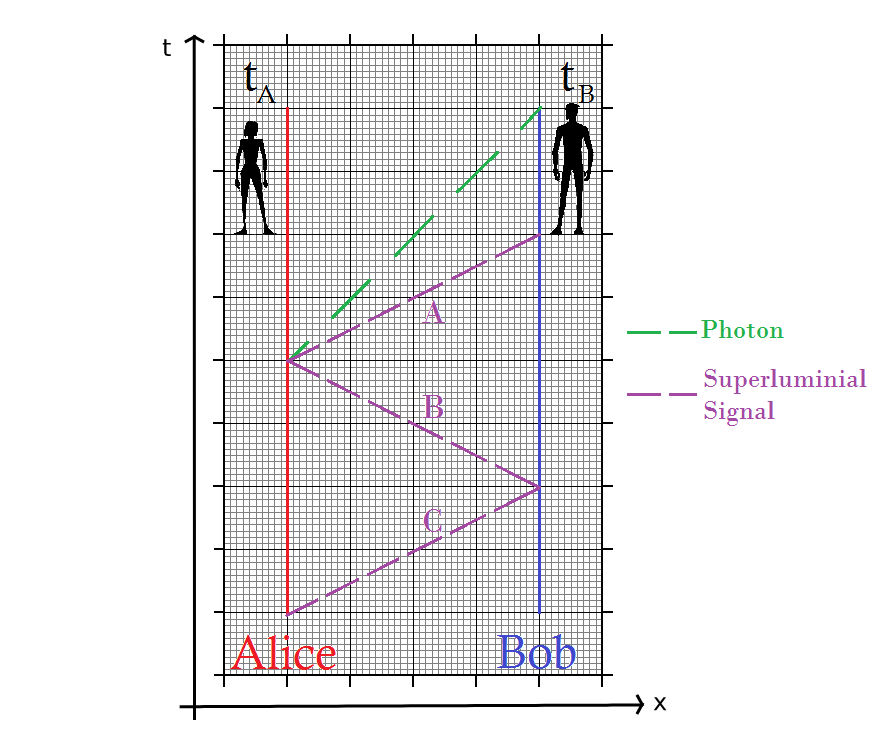
\includegraphics[width=12cm]{special-relativity.png}
\centering
\caption{Diagram Minkowskega. Diagram prikazuje komunikacijo med Alice in Bobom. Čas po vertikalni osi, razdalja po horizontalni. \cite{marcocerezoEntanglementHowIt2015}}
\label{fig:minkowski}
\end{figure}

\par
Da superluminalna komunikacija zares omogoča komunikacijo v preteklost, lahko potrdimo tudi matematično. Z $A - B$ označimo razdaljo med planetoma $A$ in $B$. Če signal potuje s hitrostjo $a$, je tedaj čas potovanja signala, merjen v inercialnem sistemu ko sta točki A in B pri miru, enak 
\begin{equation} \label{eq2}
\Delta t=t_{1}-t_{0}=\frac{B-A}{a}.
\end{equation}
Velja, da je dogodek A (oddaja signala) vzrok dogodka B (prejem signala). Za opazovalca v nekem drugem inercialnem sistemu, ki se giblje s hitrostjo $v$, lahko čas prejema signala v B izračunamo s pomočjo Lorentzove transformacije, kjer je $c$ hitrost svetlobe. Tedaj velja 
\begin{equation} \label{eq3}
\begin{split}
\Delta t' & =t'_{1}-t'_{0}=\frac{t_{1}-vB/c^{2}}{\sqrt{1-v^{2}/c^{2}}}-\frac{t_{0}-vA/c^{2}}{\sqrt{1-v^{2}/c^{2}}}\\
 & =\frac{1-av/c^{2}}{\sqrt{1-v^{2}/c^{2}}}\Delta t.
\end{split}
\end{equation}
Precej preprosto lahko pokažemo, da lahko za vrednosti $a > c$ izberemo tak $v$, da ima koeficient pred $\Delta t$ negativen predznak. To se zgodi že, če uporabimo $a = c^2 / (1 \, \frac{\text{m}}{\text{s}}) $ in $v = 2 \, \frac{\text{m}}{\text{s}}$. Z drugimi besedami - v tem inercialnem sistemu se je dogodek B zgodil še pred dogodkom A. Einstein je leta 1907 zaključil, da, čeprav v tem izrazu ne vidi nobene logične kontradikcije, je takšen rezultat kontradiktoren vsem našim izkušnjam iz realnega življenja. To pa v dovoljšnji meri dokazuje, da je primer, ko je $a > c$, nemogoč. \cite{TachyonicAntitelephone2022a}

\subsubsection{Komunikator FLASH}

\par Nick Herbert je leta 1982 predlagal shemo superluminalnega komunikatorja FLASH (Slika \ref{fig:flash}), katerega osnova je prepleten par fotonov (EPR par). Za komunikacijo uporablja dejstvo, da ima meritev enega izmed prepletenih fotonov takojšnji učinek na drugega.

\begin{figure}[h]
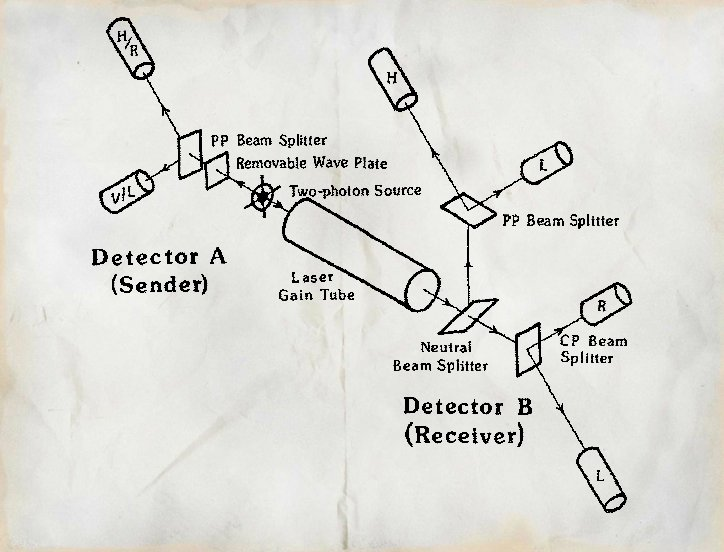
\includegraphics[width=12cm]{flash.jpg}
\centering
\caption{Originalna shema komunikatorja FLASH. \cite{herbertFLASHSuperluminalCommunicator1982}}
\label{fig:flash}
\end{figure}
\par Par prepletenih fotonov ustvarimo v dvofotonskem izviru in jih pošljemo v smeri dveh opazovalcev, npr. Alice in Bob. Stanje dveh fotnov je podano v rotacijsko invariantnem stanju
\begin{equation}
\frac{| HH \rangle + | VV \rangle}{\sqrt{2}},
\end{equation}
kjer sta $H$ in $V$ horizontalna in vertikalna polarizacija. Enako prepleteno stanje bi lahko zapisali tudi v bazi krožne polarizacije in sicer kot
\begin{equation}
\frac{| RR \rangle + | LL \rangle}{\sqrt{2}},
\end{equation}
kjer sta $R$ in $L$ desna in leva polarizacija. Ko Alice prejme svoj foton, mu lahko izmeri eno izmed dveh polarizacij, tj. linearno ali krožno. Tedaj bo tudi Bobov foton kolapsiral v linearno ali krožno polarizacijo. Bob svoj foton pred meritvijo pošlje v lasersko pomnoževalko ("Laser Gain Tube"), ki iz $n$ fotonov naredi $4n$ enako polariziranih fotonov. Bob razdeli fotonski curek na 4 dele po $n$ fotonov in izmeri polarizacije $H$, $V$, $R$ in $L$. Rezultati meritev so tedaj kot v Tabeli \ref{tab:bob}. Vse kar mora Bob sedaj storiti, je pogledati kateri izmed njegovih detektorjev je detektiral 0 fotonov. S tem izve, v kateri bazi je merila Alice. S tem v trenutku meritve (torej hipno) prejme 1 bit informacije. Po drugi strani pa smo že prej pokazali, da takšna hipna komunikacija ni možna. Kje se torej skriva napaka te sheme? \cite{marcocerezoEntangledParticlesFaster2015}
\par
Ob objavi Herbertovega članka je bilo dobro znano, da imajo izhodni fotoni iz laserske fotopomnoževalke enako polarizacijo kot vhodni. Vendar pa je Herbert spregledal, da lahko stanje npr. $| H \rangle$ zapišemo kot superpozicijo stanj $| R \rangle$ in $| L \rangle$:
\begin{equation}
| H \rangle = \frac{| R\rangle + | L \rangle}{\sqrt{2}}.
\end{equation} 
Laserska fotopomnoževalka v tem primeru dejansko pomnoži stanja $| R \rangle$ in $| L \rangle$, vsakega z verjetnostjo $1/2$. Torej na izhodu dobimo $2n$ fotonov v stanju $| R \rangle$ in $2n$ fotonov v stanju $| L \rangle$. Rezultat Bobovih meritev bi bil tedaj vedno (in neodvisno od originalne polarizacije, ki jo izmeri Alice) enak $n/2$ fotonov za vse 4 polarizacije H, V, L in R. \cite{marcocerezoEntangledParticlesFaster2015}

\begin{table}[]
\centering
\begin{tabular}{|l|l|l|l|l|}
\hline
\textbf{Alice izmeri} & \textbf{Bob - H} & \textbf{Bob - V} & \textbf{Bob - R} & \textbf{Bob - L} \\ \hline
H                     & $ 1 $            & $ 0 $            & $ 1/2 $ & $ 1/2 $ \\ \hline
V                     & $ 0 $            & $ 1 $            & $ 1/2 $ & $ 1/2 $ \\ \hline
R                     & $ 1/2 $          & $ 1/2 $          & $ 1 $   & $ 0 $   \\ \hline
L                     & $ 1/2 $          & $ 1/2 $          & $ 0 $   & $ 1 $   \\ \hline
\end{tabular}
\caption{Tabela rezultatov meritev. Žarek $4n$ fotonov razdelimo na 4 dele. Tabela prikazuje kolikšen delež $n$ fotonov, ki potujejo na posamezen detektor, bo detektiran pri Bobu glede na polarizacijo originalnega fotona.}
\label{tab:bob}
\end{table}

\par Napaka sheme torej leži v predpostavki, da lahko kloniramo naključno kvantno stanje.

 \subsection{Formulacija in dokaz}
 
 Iz prejšnjih ugotovitev lahko sedaj formuliramo izrek in ga tudi formalno dokažemo \cite{nielsenQuantumComputationQuantum2012}.

 
\begin{remark} V kvantni mehaniki ni mogoče ustvariti neodvisne in identične kopije poljubnega neznanega kvantnega sistema. 
\end{remark}

\begin{proof}
Predpostavimo, da imamo delujočo napravo za kvantno kloniranje. Naprava ima dve reži označeni z A in B. Reža A je podatkovna reža (vhod), v katero vstavimo kvantni sistem, ki ga želimo klonirati. Sistem mora biti reprezentabilen z valovno funkcijo $| \psi \rangle$ (tj. zahtevamo, da je vhodno stanje čisto). Reža B je naslovna reža (izhod). Predpostavimo, da za vse namene kloniranja v reži B začnemo s standardno valovno funkcijo, ki jo lahko reprezentiramo s $| s \rangle$. Tedaj je začetno stanje naprave za kloniranje
\begin{equation}
| \psi \rangle \otimes | s \rangle.
\end{equation}
Postopek kloniranja simboliziramo z uporabo operatorja unitarne časovne evolucije $U$ (želimo namreč ohranjati verjetnost/skalarni produkt). Zanj velja, da iz začetnega stanja naprave ustvari sledeče
\begin{equation}
| \psi \rangle \otimes | s \rangle \xrightarrow[\text{}]{\text{U}} U(| \psi \rangle \otimes | s \rangle) = | \psi \rangle \otimes | \psi \rangle.
\end{equation}
Predpostavimo, da opisani postopek deluje za dve stanji reprezentabilni z valovnimi funkcijami $| \psi \rangle$ in $| \varphi \rangle$. Tedaj dobimo 

\begin{equation}
\begin{split}
U(| \psi \rangle \otimes | s \rangle) = | \psi \rangle \otimes | \psi \rangle
\\U(| \varphi \rangle \otimes | s \rangle) = | \varphi \rangle \otimes | \varphi \rangle.
\end{split}
\end{equation}
V nadaljevanju vzamemo zgornji dve enačbi in izračunamo notranji produkt za levo in desno stran
\begin{equation}
\langle \; U(| \psi \rangle \otimes | s \rangle) \, , \, U(| \varphi \rangle \otimes | s \rangle) \; \rangle = \langle \; | \psi \rangle \otimes | s \rangle \, , \, | \varphi \rangle \otimes | s \rangle \; \rangle = \langle \psi, \varphi \rangle \, \langle s, s \rangle = \langle \psi, \varphi \rangle
\end{equation}
\begin{equation}
\langle \; | \psi \rangle \otimes | \varphi \rangle \, , \, | \psi \rangle \otimes | \varphi \rangle \; \rangle = \langle \psi, \varphi \rangle \, \langle \psi, \varphi \rangle = \left( \langle \psi, \varphi \rangle \right)^2.
\end{equation}
Rezultata enačimo in dobimo
\begin{equation}
 \langle \psi, \varphi \rangle = \left( \langle \psi, \varphi \rangle \right)^2.
\end{equation}
Vidimo, da imamo enačbo oblike $x = x^2$, ki ima le dve rešitvi, $x = 0$ in $x = 1$. Rezultat si interpretiramo takole: če bi takšna naprava lahko uspešno klonirala vsaj dve valovni funkciji $| \psi \rangle$ in $| \varphi \rangle$, tedaj mora veljati, da je $ | \psi \rangle = | \varphi \rangle$ ali pa sta valovni funkciji $| \psi \rangle$ in $| \varphi \rangle$ ortogonalni. Iz teoretičnega rezultata zaključimo, da naprave za popolno kloniranje poljubnih neznanih kvantnih sistemov ni mogoče ustvariti.
\end{proof}
 
\section{Kvantni denar} 

Izrek o prepovedi kloniranja postavi kar nekaj omejitev za nastajajoče kvantne tehnologije. Hkrati pa tudi odpira nove, prej nedosegljive možnosti uporabe. Ena izmed njih (in hkrati glavna tema našega seminarja) je shema t.i. kvantnega denarja. Le-ta z uporabo izreka o prepovedi kloniranja uvaja koncept (tudi v teoriji) neponaredljivega fizikalnega sistema, če njegovih lastnosti v naprej ne poznamo.

\begin{figure}[H]
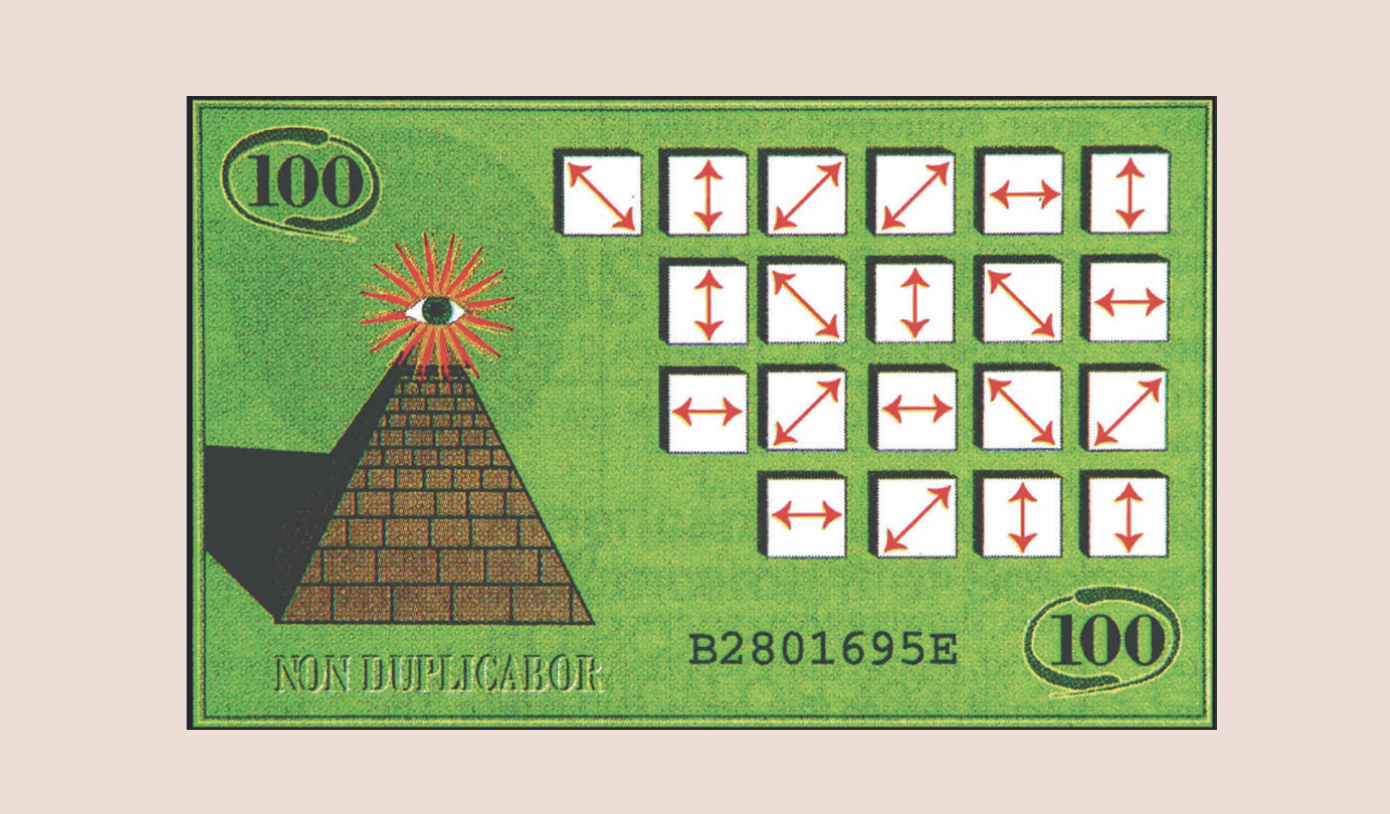
\includegraphics[width=12cm]{qmon.png}
\centering
\caption{Ilustracija kvantnega bankovca. Papirnat bankovec na sliki je opremljen z različno polariziranimi kvantnimi spominskimi celicami in serijsko številko. \cite{aaronsonQuantumMoney2012}}
\label{fig:qmoney}
\end{figure}

\subsection{Delovanje sheme}

Shemo kvantnega denarja je leta 1983 v svojem članku konceptualno opisal Stephen Wiesner \cite{wiesnerConjugateCoding1983}. Kot ilustrirano na Sliki \ref{fig:qmoney}, je vsak bankovec opremljen s serijsko številko in nizom kvantnih sistemov dolžine $N$, ki jih pripravimo v določeni (verjetno naključni) konfiguraciji $| \$_i \rangle$, $1 \le i \le N$. Naloga izdajatelja takih bankovcev je, da za vsak kvantni bankovec na varnem mestu shrani slovar serijskih številk in pripadajočo konfiguracijo $| \$_i \rangle$ za $\forall \, i$ (skrivni ključ). Varnost sistema se skriva v tem, da ponarejevalec ne ve, v kateri bazi vrne meritev sistema $| \$_i \rangle$ enoličen rezultat. Torej bo pri meritvi lahko naredil napako in jo izvedel v napačni bazi. Napačno stanje kubita bo nato zapisal na ponarejeni bankovec, kar bo pri preverjanju v banki, ki zaporedje pravilno izbranih baz pozna, detektirano. Ker je na bankovcu $N$ kvantnih sistemov, verjetnost za popolno kopijo celotnega niza pada eksponentno z $P^N \rightarrow 0$. $P$ predstavlja verjetnost, da posamezen kubit na ponarejenem bankovcu pri preverjanju producira pravilen rezultat. Dodatno zahtevamo še $0 < P < 1$. Za preprost poskus ponarejanja, kjer ponarejevalec med ponarejanjem nima dostopa do validacije bankovca, je bilo leta 2012 v \cite{molinaOptimalCounterfeitingAttacks2012} pokazano, da za $P$ ustreza vrednost $(3/4)$.

\subsection{Izbira baze za meritev}

\par Kaj pomeni izbira baze, lahko fizikalno še malo bolje razložimo. Kot opisano v točki \ref{kubit}, je možno vsak kubit reprezentirati s točkami na Blochovi sferi kot prikazano na Sliki \ref{fig:bloch}. 

\begin{figure}[H]
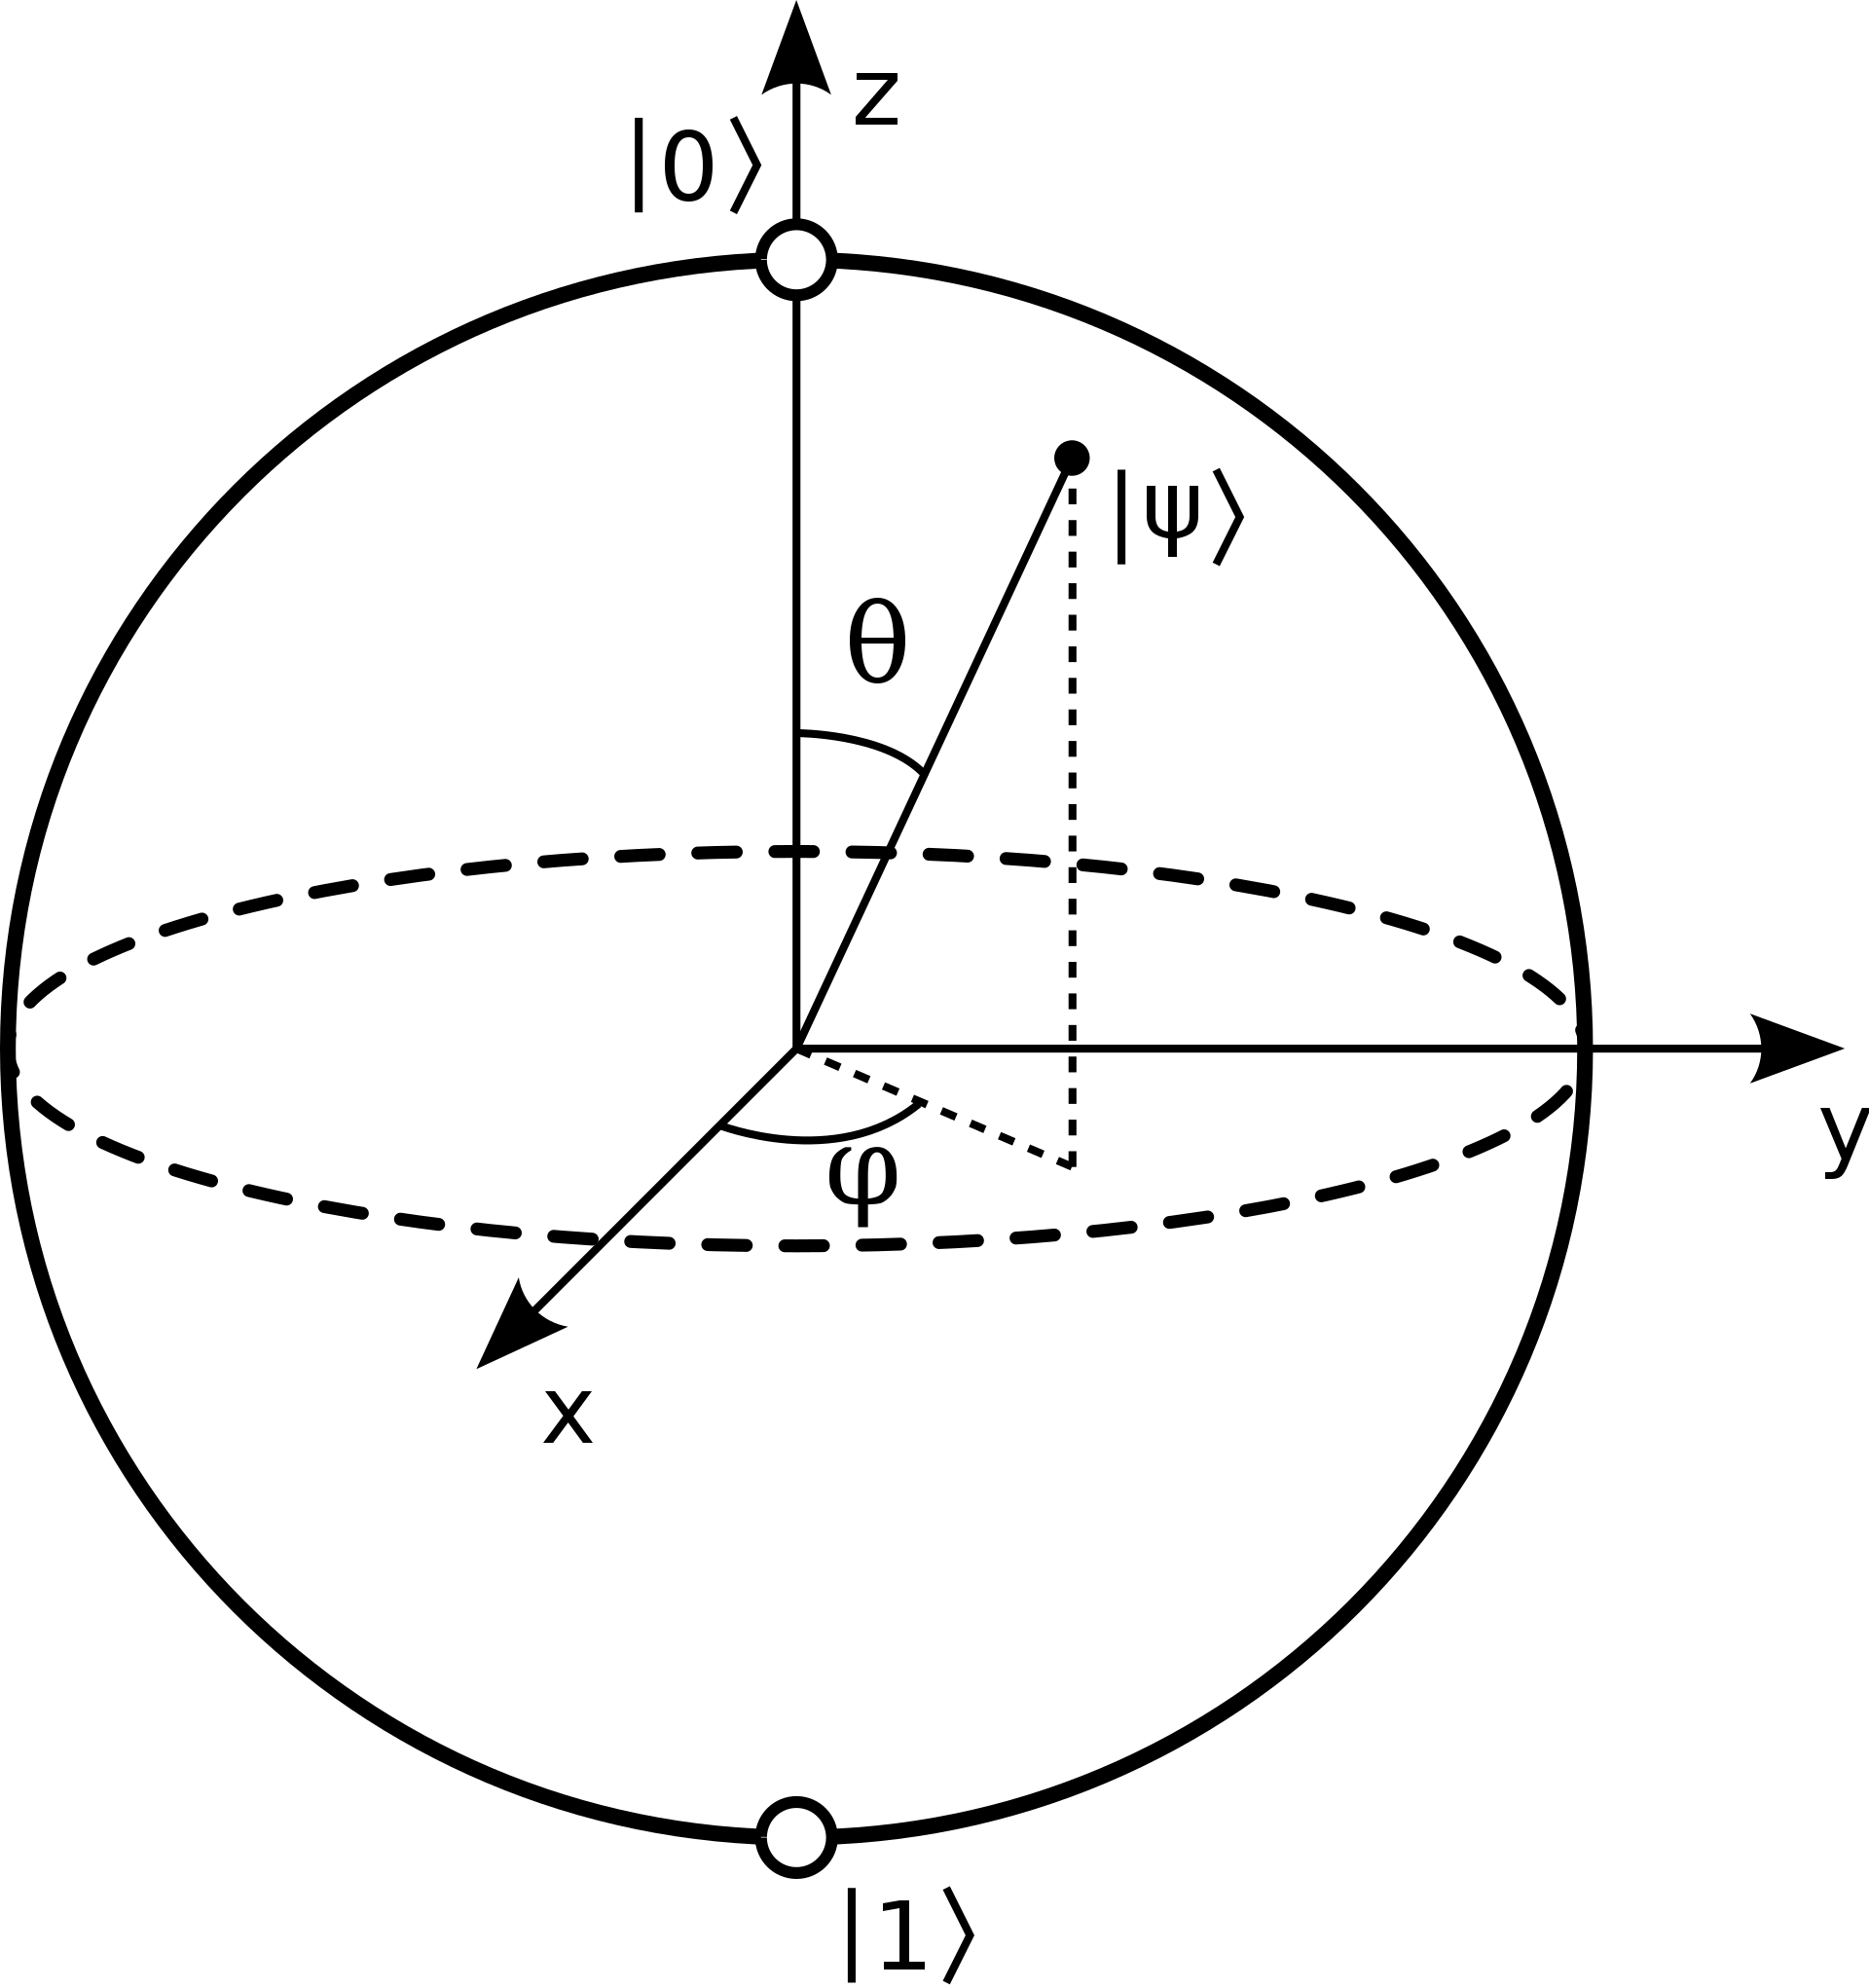
\includegraphics[width=6cm]{bloch.png}
\centering
\caption{Blochova sfera. V smeri $z$ sta definirani stanji $| 0 \rangle$ in $| 1 \rangle$. \cite{BlochSphere2023}}
\label{fig:bloch}
\end{figure}

V smeri $z$ definiramo stanji $| 0 \rangle$ in $| 1 \rangle$, ki predstavljata npr. spin dol in gor v smeri $z$. Vemo, da lahko spin merimo tudi v smeri $x$ in $y$, odvisno od orientacije Stern-Gerlachove naprave. Tedaj bi želeli zapisati tudi valovno funckcijo takšnega sistema. Pri tem si lahko pomagamo z enačbo \ref{blocheq} in vanjo vstavimo primerne kote $\theta$, $\varphi$ za bazo v smereh $x$, $y$ in $z$. Iz enačbe \ref{blocheq} tedaj dobimo 6 različnih normiranih valovnih funkcij (enačba \ref{eigenvectors}). Vemo, da ima spin 2 lastni vrednosti, in sicer $\pm 1$. Tedaj so matrični operatorji, ki ustrezajo tem lastnim vrednostim in lastnim vektorjem kar Paulijeve matrike $\sigma_x$, $\sigma_y$, $\sigma_z$. \cite{PauliMatrices2023}

\begin{equation}
\label{eigenvectors}
{\displaystyle {\begin{aligned}\psi _{x+}&={\frac {1}{\sqrt {2\,}}}{\begin{bmatrix}1\\1\end{bmatrix}}\;,&\psi _{x-}&={\frac {1}{\sqrt {2\,}}}{\begin{bmatrix}1\\-1\end{bmatrix}}\;,\\\psi _{y+}&={\frac {1}{\sqrt {2\,}}}{\begin{bmatrix}1\\i\end{bmatrix}}\;,&\psi _{y-}&={\frac {1}{\sqrt {2\,}}}{\begin{bmatrix}1\\-i\end{bmatrix}}\;,\\\psi _{z+}&={\begin{bmatrix}1\\0\end{bmatrix}}\;,&\psi _{z-}&={\begin{bmatrix}0\\1\end{bmatrix}}~.\end{aligned}}}
\end{equation}

\par Če torej naš kvantni sistem pripravimo v stanju $\psi_{x+}$ in merimo v smeri $x$, izmerimo lastno vrednost $+1$. V kolikor merimo ta isti sistem v smeri $z$ ali $y$, izmerimo lastno vrednost $+1$ z verjetnostjo $1/2$ in $-1$ z verjetnostjo $1/2$. Z drugimi besedami: ob meritvi dobimo enoličen rezultat le, če merimo v smeri lastnega vektorja valovne funkcije, torej moramo valovno funkcijo že od začetka poznati. 

\subsection{Pomanjkljivosti in ranljivosti}

Ena izmed poglavitnih težav Wiesnerjeve sheme kvantnega denarja je odvisnost od banke za preverjanje avtentičnosti bankovca. Banka mora biti vključena pri vsaki izmenjavi bankovca, saj bi z razkritjem skrivnih ključev na bankovcih padla celotna varnostna shema. Obstajata še dve pomanjkljivosti: relativno velika dolžina skrivnih ključev in ranljivost na interaktivne napade. V \cite{brodutchAdaptiveAttackWiesner2016} so leta 2016 pokazali, da lahko samo z večkratno verifikacijo istega bankovca in metodo, ki bazira na kvantnem preizkuševanju (test za bombe Elitzurja in Vaidmana), uspešno ponaredijo bankovec. Kot edina rešitev se tukaj pokaže ponovna izdaja bankovca ob vsaki verifikaciji (in s tem povezano večanje velikosti skrivnega ključa).
\par Zadnji napaki se da odpraviti, še vedno pa ostaja prva. Zato je glavni cilj nadaljnjih raziskav razvoj protokola t.i. kvantnega denarja z uporabo javnih ključev. Analogno s klasično simetrično kriptografijo, originalna Wiesnerjeva shema ustreza kvantnemu denarju z zasebnim ključem, saj lahko avtentičnost preveri le banka. Kvantni denar z javnim ključem pa bi analogno asimetrični klasični kriptografiji omogočal verifikacijo vsakomur. Ena izmed poglavitnih težav te nadgrajene sheme izvira že iz kvantnega denarja z zasebnimi ključi. Z večkratnim verificiranjem lahko ponarejevalec pridobi dodatne informacije o stanju kvantnega sistema, ki ga želi klonirati. V članku \cite{aaronsonQuantumMoneyHidden2012} avtorji predlagajo sistem kvantnega denarja z zasebnim ključem, ki omogoča neomejeno verifikacij in še vedno ostaja varen, kot tudi nov varen sistem kvantnega denarja z javnim ključem. 

\subsection{Decentraliziran kvantni denar}

Na podlagi sheme kvantnega denarja z javnim ključem \cite{aaronsonQuantumMoneyHidden2012} so v delu tudi naprednejše sheme, ki namesto centralne banke v vlogo verifikatorja postavijo decentraliziran sistem validatorjev. V članku Kvantni Bitcoin avtorji (\cite{jogenforsQuantumBitcoinAnonymous2019}) nadgradijo protokol veriženja blokov Bitcoin, ki ga uporabijo za verifikacijo in izdajo fiksne količine fizičnih kvantnih bankovcev kot primer decentralizirane valute, ki je ne nadzoruje nobena banka, temveč decentraliziran sistem validatorjev.   

\subsection{Fizična realizacija}
Trenutno ne obstaja nobena praktična in cenovno ugodna tehnologija, ki bi omogočala masovno implementacijo katere koli prej opisane sheme. Za to namreč potrebujemo t.i. kvantni pomnilnik - komponento analogno npr. pomnilniku FLASH - ki je za daljše časovno obdobje sposobna shraniti stanje kubita in je odporna na motnje iz okolice. Trenutno je to eno izmed bolj aktivnih področij raziskav. Avtorjem nedavnega članka \cite{RobustMultiqubitQuantum} je uspelo ustvariti dvokubitni register, ki lahko pri temperaturi 1.5 $K$ shrani kvantno stanje fotonov za nekaj več kot 2 sekundi.  

\section{Zaključek}

V okviru tega seminarja smo preleteli osnovne koncepte kvantne informatike, dokazali izrek o prepovedi kloniranja in pokazali njegovo uporabo na konceptu kvantnega denarja, ki rešuje praktičen problem ponarejanja. Poleg kvantnega denarja so aktivna področja raziskav tudi: super gosto kodiranje, kvantna izmenjava ključev (QKD), kvantne kode za popravljanje napak, kvantni algoritmi, itd. Zanimvo bo videti, kako hitro nam bo uspelo zapletene kvantne naprave iz laboratorijev preseliti v naš vsakdan.

\pagebreak
       
 \printbibliography[heading=bibintoc,title={Literatura}]
    \end{document} 